
\thispagestyle{empty}

% Incomplete compensation for fixation depth in eye movement driven self-motion perception
% Incomplete compensation for fixation depth for eye movement induced self-motion perception
% Lateral translation perception is modulated by eye movements that are partially scaled for viewing depth. 
% Translational motion perception from eye movements is partially scaled by viewing depth

\chapter{Translation perception is modulated by eye movements that are partially scaled by fixation depth}
\chaptermark{}

\newpage

\small {\bf Abstract}
Previously, we have shown that the eye movements that typically accompany self-motion are used to augment self-motion perception. As fixation depth modulates the amplitude of these eye movements, it should be taken into account for a veridical oculomotor estimate of self-motion. To investigate whether the brain compensates for fixation depth, we had  participants ($n = 8$) judge self-motion during different eye movement conditions in the absence of full-field optic flow.  In a 2-AFC task, participants indicated whether the second of two successive passive lateral whole-body translations was longer or shorter than the first. At the start of each movement participants fixated either a nearby or a far away target, which was either body stationary or world stationary during the translation interval. Results show that the perceived translations were shorter for nearby world-fixed gaze compared to far away world-fixed gaze, indicating that eye movements are not properly scaled in self-motion perception. Together with the observation that self-motion perception is not affected by the depth of a body stationary fixation target, we conclude that eye movements are merely a rudimentary cue to self-motion, with a compensation for fixation depth that is partial at best.

\vfill

\noindent\underline{ \hspace{4cm} }

\noindent This chapter is being prepared for publication \newline
\noindent {\bf Clemens, I.A.H.}, Selen, L.P.J., MacNeilage, P.R. and Medendorp, W.P. \citeyear{clemens2015b}. %Title. \emph{Journal}, volume(issue): from-to. \newline

\newpage

\section{Introduction}

An accurate internal estimate of self-motion is required to navigate effectively through a complex three-dimensional environment. The vestibular system as well as optic flow provide essential information about self-motion \cite{gibson1955, benson1986, harris2000, israel1989, angelaki2005, carriot2013, chen2010}. During navigation, however, the eyes typically move to maintain visual acuity on important objects. These eye movements disturb the optic flow patterns. Using the oculomotor signal, the brain is able to account for these disturbances by internally separating optic flow into two components, one caused by self-motion and the other by eye movement \cite{warren1988, royden1992, freeman1998, lappe1999}.

When the eyes track world-centered objects, their angular displacement is directly related to the size of the motion of the observer \cite{schwarz1989, paige1998, mchenry2000, medendorp2002}. Because  the majority of fixations are on world-stationary  objects, we recently proposed that these tracking eye movements could also be used as a self-motion cue, in addition to optic flow and vestibular signals. To test this hypothesis, we compared self-motion perception in the absence of full-field optic flow during passively induced whole-body translations \cite{clemens2015a}. Our results showed that self-motion is underestimated during body-centered fixations (in which the eyes remain stationary in their orbits) compared to fixations on world-stationary objects (in which the eyes must move to maintain fixation).

Geometrically, eye movements that keep fixation on a world-centered target during lateral whole body translation (i.e. the linear vestibulo-ocular reflex; LVOR), must scale with fixation depth \cite{angelaki2004}. When fixating body-centered targets these eye movements must be suppressed irrespective of fixation distance \cite{angelaki2004}. Conversely, when fixating world-centered targets, the brain must internally scale the ensuing eye movement by fixation distance to serve as an adequate self-motion cue. Because we did not manipulate fixation distance in our previous study, we could not dissociate whether eye movements are used as a rudimentary cue for self-motion (i.e. without taking fixation depth into account), or are properly scaled in the mechanisms for self-motion perception.

In the present study, we investigate how fixation distance influences perception of self-motion during passive lateral translation. Using a psychophysical approach, participants had to indicate whether the second body displacement of two one-second translation intervals was smaller or longer than the first. We show that translation amplitude is perceived smaller when fixating a far compared to a nearby world-centered target, indicating that eye movements are not properly scaled in self-motion perception. Together with the observation that self-motion perception is not affected by the depth of a body-centered fixation target, we conclude that eye movements are merely a rudimentary cue to self-motion, with a compensation for fixation depth that is partial at best.

\section{Materials and methods}

\subsection{Participants}

Eight naïve participants (three male, five female), aged between 22 and 29 years, gave written informed consent to participate in the study. They were all free of any known vestibular or neurological disorder and had normal or corrected-to-normal visual acuity. Participants never received any feedback about their performance. The present study was part of a larger study on the effects of eye movements on self-motion perception, some of the results of which were described in our recent report \cite{clemens2015a}. Details about the setup and methods have been described extensively in that report as well. Here we provide only a brief summary.


\subsection{Experimental setup}

Participants were seated on a motorized linear sled with their body and head restrained such that the inter-aural axis aligned with the motion axis. The sled laterally translated participants following a minimum jerk profile of fixed duration (1s) and amplitudes ranging from 1 to 27 \si{\centi\metre}. Auditory cues were suppressed using white noise presented through in-ear head-phones. Experiments were conducted in complete darkness except for visual fixation points, projected by body- or world-fixed laser pointers on a black bar, either 50 or 200 \si{\centi\metre} in front of the sled and at eye level. Eye movements were recorded at 500Hz using an EyeLink II (SR Research, Kanata, Canada) system. Eye position was calibrated before each session using 11 evenly spaced calibration points ranging from -22 to 22 degrees.


\subsection{Paradigm}

We used a two-alternative forced choice (2-AFC) task to study the influence of fixation depth on the perception of linear translation. We tested two fixation depths: near (50 cm) and far (200 \si{\centi\metre}) and two different eye fixation conditions: world-, and body-fixed fixation. A trial contained two sequential motion intervals of equal duration (1s), with the motion in the same direction (either leftward or rightward). Fixation condition (world, or body-fixed) was the same in both intervals, but a different fixation depth was presented in each. Participants had to judge whether the translation during the second motion interval was longer or shorter than in the first motion interval.

\begin{figure}
    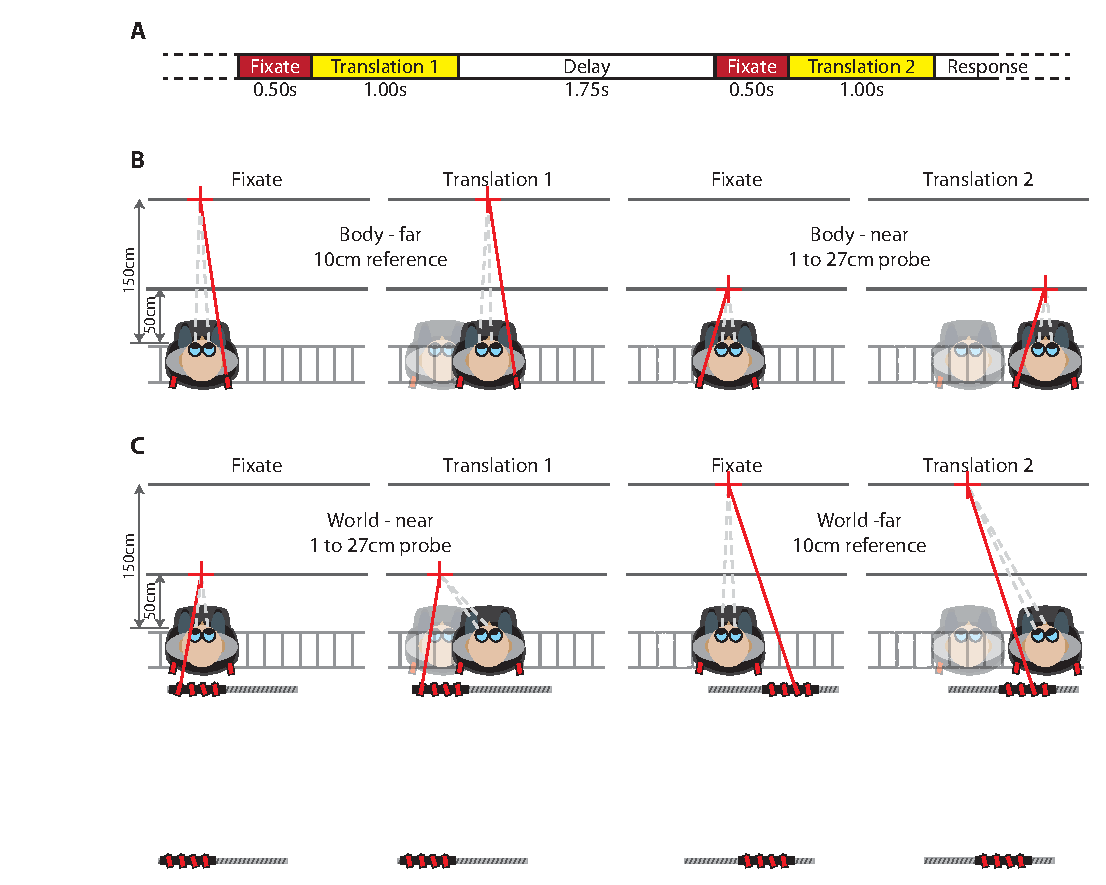
\includegraphics[width=1.0\textwidth]{src/paper4/paper4_figure1.eps}

    \caption{...}
    \label{p4:fig1}    
\end{figure}
 
The timing of a single trial is shown in \figref{p4:fig1}A. Each trial started with the onset of a central fixation point (i.e. aligned between the eyes) for 0.5s. Subsequently, the first 1s motion interval commenced, during which the fixation type which was at on the the two depths, remained stationary (world) or moved along with the participant (body). Subsequently a 1.75s delay followed in which the participant was kept in complete darkness. Then, the central fixation point reappeared, followed 0.5s later by a second 1s translation interval, with the same fixation condition but with fixation point at the other depth as in the first interval. Finally, the participant responded by moving a 1-dimensional joystick away from (longer) or towards (shorter) the body. Top-view illustrations of body-centered and world-centered trials are shown in Figures 1B and 1C respectively.

\begin{table}
    \begin{tabular}{llll}
    Comparison & Reference & 1st interval & Direction \\
    \hline
    Body & Near & Reference & Right \\
    Near vs. far & & & Left \\    
    & & Probe & Right \\
    & & & Left \\
    \cline{2-4}
	& Far & Reference & Right \\
    & & & Left \\    
    & & Probe & Right \\
    & & & Left \\
    \hline
    World & Near & Reference & Right \\
    Near vs. far & & & Left \\    
    & & Probe & Right \\
    & & & Left \\
    \cline{2-4}
	& Far & Reference & Right \\
    & & & Left \\    
    & & Probe & Right \\
    & & & Left \\
    \end{tabular}

    \caption{List of the 2 main comparisons that we tested. The (10cm) reference movement was presented in either the first or the second interval. We also manipulated movement direction (leftward vs rightward) yielding a total of 16 trial types.}

    \label{p4:tab1}
\end{table}

Across trials, we varied fixation distance, as well as the order of reference and probe, giving a total of four variations per condition (see \tabref{p4:tab1}). Movement direction (either leftward or rightward) alternated between consecutive trials. The size of the probe translation was adaptively chosen based on the participants' earlier responses (Psi method; {Kontsevich:1999tg}) to determine the point of subjective equality. This was done separately for all 16 trial types (2 main conditions x 2 reference stimuli x 2 reference/probe orders x 2 movement directions; see Table 1). A total of 25 trials were collected per trial type yielding a total of 200 trials for each of the two main conditions.

Trials were presented in two one-hour sessions. To prevent dark adaptation, we turned on the lights for 5s after each block of 8 trials, and for at least 30 s after every 2 blocks. Each of the 16 unique trial types were presented once every 2 blocks. After each block, the adaptive procedure determined which translation size to test in the following block. To increase the number of data-points available to the adaptive psychometric procedure at the beginning of the experiment, we collapsed across movement direction and reference order for the first 10 trials. After that, the procedure ran separately for each of the 16 distinct trial types.

\subsection{Data analysis}

For each combination of the two main conditions and the two reference/probe orders (see \tabref{p4:tab1}), we quantified the perceived probe translation by calculating the probability the probe translaton was pereived longer than the reference translation as a function of actual probe translation. We used a maximum likelihood fit of a cumulative Gaussian function to summarize the psychometric data:

\begin{equation}
\label{p4:eq1}
P(x) = \lambda + (1 - 2\lambda) \frac{1}{\sigma \sqrt{2\pi}} \int_{-\infty}^{x}{e^{-(y-\mu)^2 / 2\sigma^2}}dy,
\end{equation}

in which $|x|$ represents the size of the probe translation. The mean of the Gaussian, PSE, represents the point of subjective equality. The slope of the curve reflects the precision ($1/\sigma$) of reference-probe discrimination performance. Parameter $\lambda$, representing the lapse rate, accounts for stimulus-independent errors caused by subject lapses or mistakes and was restricted to small values ($\lambda < 0.06$). Fits were performed using the Psignifit toolbox {Wichmann:2001ud, Wichmann:2001wa}.
For each trial type (see \tabref{p4:tab1}), we also quantified eye movements, corrected for drift based on initial fixation. We discarded trials containing blinks as well as trials where the final eye position was more than two standard deviations away from the condition average. In total, about 12\% of all trials were discarded. After rejecting trials, we computed the average ratio between the actual, , and ideal eye movement angle that would have occured in the world-fixed fixation condition (Equation 2). This ideal eye movement angle is computed by taking the arc-tangent of the actual translation distance, , divided by the fixation depth, . We computed this ratio, , for every condition c (see Table 1). Note that for body fixation the normalized eye movement would be  and for world fixation would be .

\begin{equation}
\label{p4:eq2}
\end{equation}

Using this ratio, , we can compute the expected eye movement,  at arbitrary translation distances, even ones we did not explicitly measure:

\begin{equation}
\label{p4:eq3}
\end{equation}

Model
Using the simple cue integration model we introduced in our previous paper (Clemens et al., 2014) as a starting point, we investigate the manner in which fixation depth is taken into account. As in our previous paper, we model the perceived distance, , as a weighted combination of a vestibular, , and oculomotor estimate of translation,  (Equation 4). 

\begin{equation}
\label{p4:eq4}
p_i = \alpha_{d_i} \hat{\varphi}_i + (1 - \alpha_{d_i}) m_i
\end{equation}

As the weighting parameter, , can depend on fixation depth,, it can explain both fixation depth depedent as well as independent effects. The exact distribution between these components can be found by analyzing the weighting parameter. If the weighting parameter is the same across all values for fixation depth , then there is no depth dependent part. Similarly, highly different parameters would indicate depth dependent effect. Further note that while we assume that that the vestibular () and oculomotor weights ( sum to one, they could sum to any arbitrary value by scaling the weights appropriately. 
By definition, the probe displacement (subscript p) is perceived as equal in length to the 10 cm reference displacement (subscript r) at the PSE, . By substituting both sides by the right hand side of Equation 4, we obtain:

\begin{equation}
\label{p4:eq5}
\alpha_{d_r} \hat{\varphi}_i + (1 - \alpha_{d_r}) m_i = \alpha_{d_p} \hat{\varphi}_i + (1 - \alpha_{d_p}) m_i + \epsilon
\end{equation}

In the present experiment, the reference displacement, , was always 10 cm and the probe displacement, , was equal to the measured PSE for the presented combination of fixation types (i.e,  in Equation 1). This model (i.e. Equation 5) was then fit to data from the body and world conditions using linear regression, finding one weight for every fixation depth (that is,  and ) that minimizes the sum of squared errors (. 
As mentioned before, these weights model both depth dependent as well as depth independent effects. Perfect compensation for fixation depth would require multiplication of the eye movement angle by the actual fixation depth, . The actual value of  used depends on the relative amount of compensation for fixation depth. This means that   and, in the specific case of our near and far targets,  and . By dividing our parameters, we remove the depth independent part  and reveal the ratio of fixation depth value used for compensation, . In case of perfect compensation the expected ratio is be , while in case of no compensation it is 1.

\section{Results}

In a recent study we have shown that eye movement signals contribute to the perception of body translation, even in the absence of optic flow \cite{clemens2015a}. Because eye rotations must be scaled by target depth ($\varphi d = T$) to serve as an adequate translation cue, we tested the effect of near versus far fixation on self-motion perception. Participants were presented with two subsequent translation movements \figref{p4:fig1} and had to judge whether the second translation was perceived longer or shorter than the first. During each interval, participants fixated either a body- or world-fixed fixation point either nearby (50 cm) or further away (200 cm).

\begin{figure}
    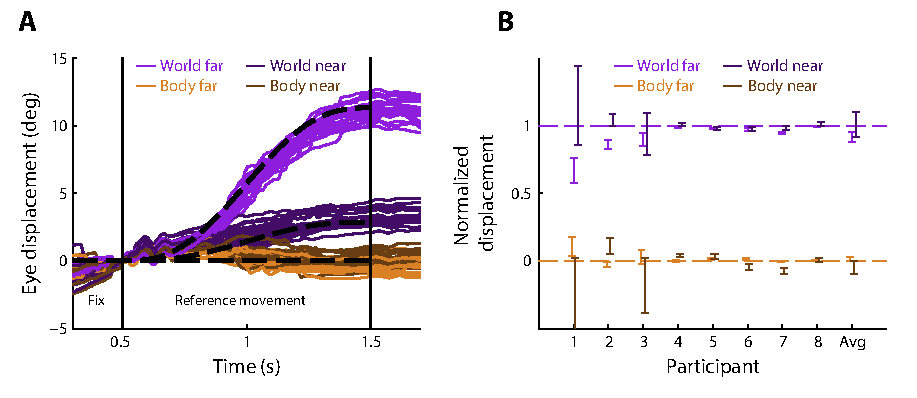
\includegraphics[width=1.0\textwidth]{src/paper4/p4_figure2.pdf}

    \caption{\panelref{A} Actual (solid lines) and ideal (dashed lines) eye movement traces of one participant in the body-fixed (brown and orange) and world-fixed conditions (purple and pink). Gaze was directed at a near (brown and purple) or far (orange and pink) target. All traces shown are for 10m reference movements. \panelref{B} [Need to decide what to put here.]}
    \label{p4:fig2}
\end{figure}

We first tested the ability of participants to follow the eye movement instruction in our paradigm. \figref{p4:fig2}A depicts exemplar eye traces for the 10cm reference translation with nearby and far fixation points in both the body and world condition. Changes in gaze are largely absent in the body near and body far conditions (brown and orange traces respectively), as required. During the world conditions, the eye movements were large when fixating nearby targets and small when fixating far away ones (purple and pink traces respectively), which reflects the geometrical constraints. 

We analyzed the eye movement data by taking the average ratio between the measured eye excursion and the geometrically required displacement were the target at a world-fixed location. \figref{p4:fig2}B shows these normalized eye displacements for all participants, which are about zero during body fixed fixations (brown and orange) and close to one in the world fixed fixations (purple and pink data points). Does the brain scale these eye movements by fixation depth in order to interpret them as a linear self-motion cue?

\begin{figure}
    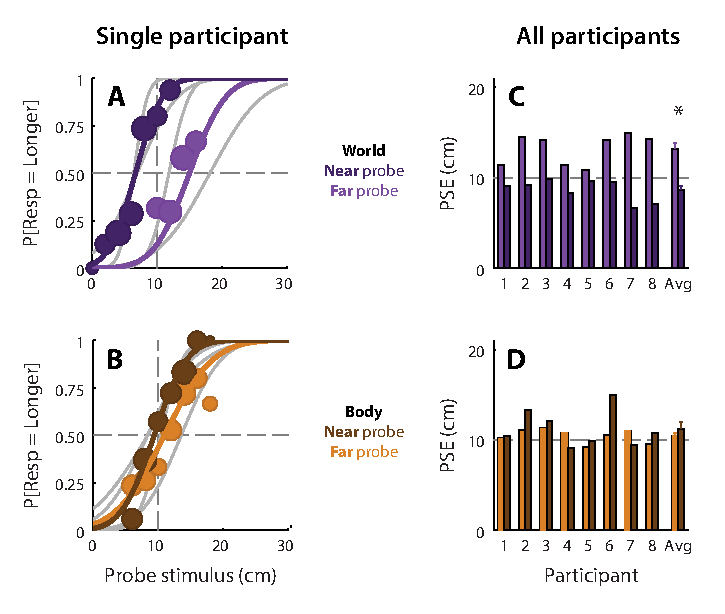
\includegraphics[width=1.0\textwidth]{src/paper4/p4_figure3.pdf}

	\caption{\panelref{A} and \panelref{B} Psychometric curves (colored lines) and associated binned data (circles) for one participant. Circle size represents the amount of trials within the bin. Psychometric curves before collapsing across reference order are shown as gray lines. \panelref{A} Body-fixed condition (brown) while fixation was either near (dark) or far (light). \panelref{B} World-fixed condition (purple) while fixation was either near (dark) or far (light).
	\panelref{C} and \panelref{D} Individual and average points of subjective equality (PSEs). Color scheme matches panels A and B.
	}
	\label{p4:fig3}
\end{figure}

To answer this question, \figref{p4:fig3} illustrates psychophysical data on self-motion perception of a single participant for the two-fixation depths in the body (\figref{p4:fig3}A) and world condition (\figref{p4:fig3}B) respectively. Lighter and darker colors indicate which fixation type was the reference translation (see figure legend). The influence of fixation distance is characterized by a shift of the psychometric functions relative to the 10 \si{\centi\metre} reference translation (i.e. the PSE). For example, the rightward shift of the pink curve in \figref{p4:fig3}B, representing the world-condition, means that with a far target a longer translation (~15 \si{\centi\metre}) was required to be perceived equivalent to a 10 \si{\centi\metre} reference translation with nearby fixation. Likewise, the leftward shift of the purple curve indicates that a shorter translation with near fixation (~6 \si{\centi\metre}) is required to be perceived the same as the 10 \si{\centi\metre} reference translation with far fixation. Together, these opposite biases suggest that translations are perceived shorter for fixations further away. The brown and orange curves in \figref{p4:fig3}A do not show such shifts, indicating that fixation depth (i.e. near versus far) has no effect in absence of eye movements (i.e. when fixating a body-fixed target during the translation).

Similar results were obtained for all participants, as shown by the individual PSEs (right column of \figref{p4:fig3}). Statistical significance of the effects of fixation depth was evaluated by comparing PSEs for the two fixation depths using a paired t-test. PSEs were significantly different in world condition, $t(7) = 5.42$, $p < 0.01$ (\figref{p4:fig3}C), but not in the body condition, $t(7) = -1.17$, $p = 0.28$ (\figref{p4:fig3}D), confirming the single subject results (\figref{p4:fig3}A, B). Thus, increasing fixation depth does not influence self-motion perception during body fixed fixations, but causes self-motion to be perceived as shorter during world-fixed fixations.

\begin{table}
    \begin{tabular}{l|lll|l}
	Participant & $\alpha_{50}$ & $\alpha_{200}$ & $\frac{d_{200}}{d_{50}}$ & $\alpha$ \\
    \hline
	1 & 0.37 & 0.25 & 1.46 & 0.27 \\
	2 & 0.51 & 0.41 & 1.25 & 0.27 \\
	3 & 0.36 & 0.30 & 1.22 & 0.35 \\
	4 & 0.14 & 0.29 & 0.49 & 0.06 \\
	5 & 0.11 & 0.04 & 2.79 & 0.13 \\
	6 & 0.49 & 0.15 & 3.34 & 0.33\\
	7 & 0.40 & 0.53 & 0.76 & 0.58 \\
	8 & 0.42 & 0.35 & 1.25 & 0.21 \\
    \end{tabular}

    \caption{Best-fit parameter values for 50 and 200 \si{\centi\metre} fixation distances, $\alpha_{50}$ and $\alpha_{200}$ respectively (see \eqnref{p4:eq5}), and their ratio, $\frac{\alpha_{200}}{\alpha_{50}} = \frac{d_{200}}{d_{50}}$, for each participant. Best-fit parameter values, $\alpha$, from our previous paper \protect\cite{clemens2015a} are included for reference.}

    \label{p4:tab2}
\end{table}

\begin{figure}
    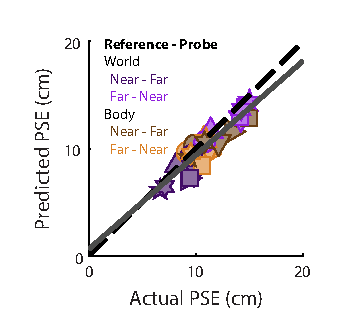
\includegraphics[width=0.5\textwidth]{src/paper4/p4_figure4.pdf}

	\caption{PSEs for all participants and the average \textpm SE. \panelref{A}  Body-fixed condition while fixation was either near (brown) or far (orange). \panelref{B} World-fixed condition while fixation was either near (purple) or far (pink).}
	\label{p4:fig4}
\end{figure}

In order to quantify how much fixation depth scales the eye movement as a linear self-motion cue, we used a simple linear model (see \nameref{p4:sec:methods}). This model explains the perceived translation distance as a weighted average of a vestibular estimate, equal to the actual translation, and an oculomotor-based estimate. 
We used two weighting parameters, $\alpha_{50}$ and $\alpha_{200}$, one per fixation depth (see \tabref{p4:tab2} for best-fit values). Using these parameters we predicted the PSEs, i.e. $m_p$ in \eqnref{p4:eq5}, and plotted them against the actually observed PSEs in \figref{p4:fig4}. The positive correlation ($\rho = 0.xx$, $p < 0.01$) between observed and predicted PSEs shows that our simple model does reasonably well in predicting perceptual performance.

\begin{figure}
    \includegraphics[width=0.5\textwidth]{src/paper4/p4_figure5.pdf}

	\caption{}
	\label{p4:fig5}
\end{figure}

By examining the ratio of these weighting parameters, we remove any depth-independent contributions. In absence of  depth scaling, i.e. when $d_{50} = d_{200}$, the ratio should be one. For perfect compensation, that is when $d_{50} = 50  \wedge d_{200} = 200$, the ratio should be $1/4$. The actual ratio between $d_{50}$ and $d_{200}$ is plotted for each participant in \figref{p4:fig5}. While two participants show moderate compensation for depth, the majority of participants show no sign of scaling of eye movements by fixation distance. This is consistent with the observation that translations are perceived shorter with far compared to near fixations in the world condition.

\section{Discussion}

% Relation to previous work / Should rewrite this paragraph!
In our previous study, we demonstrated that oculomotor signals play a substantial role in the perception of self-motion, even in the absence of optic flow or any other visual stimulation \cite{clemens2015a}. Although the vestibular system provided the most significant contribution, oculomotor signals were shown to account for about 20\% of the overall percept. Because these experiments were performed with a single fixation depth, it was not clear whether the brain weighted the oculomotor signal in a depth-dependent manner when using it as a translation cue, or merely uses the signal as a rudimentary cue to self-motion. In the present study we tested between these two possibilities.

% Basic observations
We assessed self-motion perception during either body- and world-centered fixation at two different fixation depths. Our results show that self-motion was underestimated when comparing far and near fixation trials in the world-centered condition, which argues against a proper scaling of the eye movement signal. Fixation depth did not influence self-motion perception during body-centered fixation (where eye movements are virtually absent).  

% Model results
To quantify the relative depth-dependent scaling of eye movements for nearby and far away fixation targets, we fitted a straightforward linear model to the perceptual responses based on the oculomotor behavior across four conditions. While two participants show partial scaling, the other six participants did not show any sign of scaling. Thus, we conclude that while oculomotor signals provide a robust clue to translation perception, they are not properly scaled by fixation depth.


\subsection{Relation to previous studies}

% Relation to Clemens, 2015
\begin{figure}
    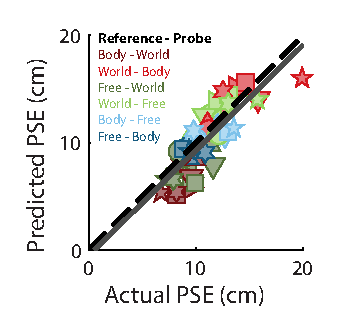
\includegraphics[width=0.5\textwidth]{src/paper4/p4_figure6.pdf}

    \caption{...}
    \label{p4:fig6}
\end{figure}

In our previous experiment we compared body-fixed to world-fixed fixations at near (50 \si{\centi\metre}) distances only \cite{clemens2015a}. We compared the parameter, $\alpha$, found in that paper with the parameters for the near condition, $\alpha_{50}$, found in the present study. \figref{p4:fig6} shows how well our $\alpha_{50}$ parameter explains the data in our previous paper, the positive correlation between the actual PSEs and those predicted using the model in this paper (stats) adds confidence to the parameter values for  presented here. The average difference between the values found here and those reported previously (see \tabref{p4:tab2}) is 12 \textpm 8 percent-points, indicating a variation of about 12\% on the contribution of the vestibular system versus that of the visual system between the present and our previous paper. While the variation might seem high, keep in mind that the two parameter values presented in this study are fitted on only four conditions, which do not overlap with the two conditions used to fit  parameter  previously.

% Relation to the VOR, e.g. Paige and Busettini
Because the LVOR is commonly thought to keep the eyes stable during linear translation (reference), it also needs to scale with fixation depth. It is therefore possible that both the LVOR and self-motion perception use the same signal. While the fixation point in our experiment causes optokinetically driven eye movements to suplement the LVOR compensation, it is known that the LVOR only partially compensates for the amount of linear translation. If the same signal is also used for self-motion perception, one would expect that, the ratio of the expected LVOR compensation at 50 and 200cm reflect the ones presented in this paper (see \figref{p4:fig5} and \tabref{p4:tab2}).

It has been shown that the relative amount of compensation, or gain, depends on fixation distance angle \cite{paige1989, busettini1994,paige1998}. When fixating far away the gain is closer to 1 compared to fixations closer by. We extrapolated the gains found by Paige, 1989 to the 50 and 200cm fixation distances in our experiment and found gains of 0.50 and 0.68 respectively.

The expected LVOR compensation based on these gains is 5.6 and 3.0 degrees for near and far fixation respectively. The ratio, 1.87, does not match either the 6 participants who do not show any sign of scaling ($\frac{d_{200}}{d_{50}} = 1.07 \pm 0.16$) or the 2 that do ($\frac{d_{200}}{d_{50}} = 3.06 \pm 0.27$), but does match the overall overage of  1.56 \textpm 0.35.

% Talk about whether perception and action employ different mechanisms?
% Check work by Merfeld
%
% Vestibular perception and action employ qualitatively different mechanisms I and II
% Merfeld, Park, Gianna-Pulin, Black, Wood, 2005
%

% -- %

% Self-motion perception; disambiguation
% Rotation perception; do not expect fixation distance to play a role

% Link to path reception during rotation, influence of instructions, depth range, and dot density:
% Li Li, William H. Warren Jr. doi:10.1016/j.visres/2004.03.008

% Experimental Brain Research doi:10.1007/s00221-009-1828-z 123
% Eye eccentricity modifies the perception of whole-body rotation
% Gaelle Quarck, Lena Lhuisset, Olivier Etart, Pierre Denise


\subsection{Alternative explanations}

In addition to the absence of scaling, another explanation is that eye movement information is integrated in a statistically optimal fashion, taking signal noise into account. In the world-fixed condition, this would mean that noisy eye movements in the far fixation are weighed less than those in the less noisy ones in the near fixation condition, giving rise to the observed difference. In this case, similar optimal integration should also occur in the body-fixed fixation condition. As no such differences between the near and far body-fixed fixation conditions have been observed, this is unlikely to be the case.  \footnote{\textbf{I do not understand the text Pieter proposed, I think it says something completely different.} While the brain should scale eye movements by fixation depth when using them as a geometrical veridical cue to translation perception, our data do not confirm this hypothesis. Does this imply that the brain does not apply any transformation to oculomotor feedback signals? It is important to realize that our analysis did not account for the fact that noise levels in the oculomotor signal could depend on fixation depth. If we would incorporate this notion in our analysis, i.e.  oculomotor signals are weighted by their noise level, it would suggest that the eye movements occurring with near fixation points are more noisy than those with a far fixation point. Our data provide no indication for this being the case. }

% FIXME: Change X and Y in paragraph below; I don't like asking questions like this.
Could the lack of scaling be explained by how participants perceive the far fixation point? Because the difference between body- and world-fixed fixation points is reduced at far fixation distances, the lack of scaling could - in theory - be explained by participants incorrectly perceiving both the body- and world-fixed far fixation points as being body-fixed. We consider this an unlikely explanation, because the target displacement associated with a world-fixed target was between X and Y degrees in our experiment, which is easily perceivable especially given that the target was foveated. This adds confidence to our claim that eye movements indeed influence self-motion perception, with moderate to no scaling for fixation depth.

\subsection{Conclusion}
% Conclusion
In summary, fixation depth is not properly taken into account, suggesting that a relatively raw eye movement signal is used in self-motion perception. While efference copies of the eye movement signals or proprioceptive feedback could be directly responsible for the perceived self-motion, it cannot be ruled out that the signals that drive the eye movements are not causing the reported effects instead.


